

\tikzset{every picture/.style={line width=0.75pt}} %set default line width to 0.75pt        

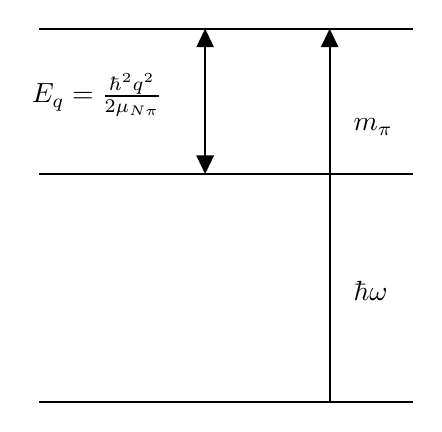
\begin{tikzpicture}[x=0.75pt,y=0.75pt,yscale=-1,xscale=1]
	%uncomment if require: \path (0,300); %set diagram left start at 0, and has height of 300
	
	%Straight Lines [id:da9050164165880492] 
	\draw    (210,200) -- (390,200) ;
	%Straight Lines [id:da595724624922532] 
	\draw    (210,90) -- (390,90) ;
	%Straight Lines [id:da8326738532712242] 
	\draw    (210,20) -- (390,20) ;
	%Straight Lines [id:da4515077860512252] 
	\draw    (350,200) -- (350,23) ;
	\draw [shift={(350,20)}, rotate = 90] [fill={rgb, 255:red, 0; green, 0; blue, 0 }  ][line width=0.08]  [draw opacity=0] (8.93,-4.29) -- (0,0) -- (8.93,4.29) -- cycle    ;
	%Straight Lines [id:da5226155750538098] 
	\draw    (290,87) -- (290,23) ;
	\draw [shift={(290,20)}, rotate = 90] [fill={rgb, 255:red, 0; green, 0; blue, 0 }  ][line width=0.08]  [draw opacity=0] (8.93,-4.29) -- (0,0) -- (8.93,4.29) -- cycle    ;
	\draw [shift={(290,90)}, rotate = 270] [fill={rgb, 255:red, 0; green, 0; blue, 0 }  ][line width=0.08]  [draw opacity=0] (8.93,-4.29) -- (0,0) -- (8.93,4.29) -- cycle    ;
	
	% Text Node
	\draw (360,140) node [anchor=north west][inner sep=0.75pt]    {$\hbar \omega $};
	% Text Node
	\draw (360,62) node [anchor=north west][inner sep=0.75pt]    {$m_{\pi }$};
	% Text Node
	\draw (205,40) node [anchor=north west][inner sep=0.75pt]    {$E_{q} =\frac{\hbar ^{2} q^{2}}{2\mu _{N\pi }}$};
	
	
\end{tikzpicture}